%%%%%%%%%%%%%%%%%%%%%%%%%%%%%%%%%%%%
% Header                           %
%%%%%%%%%%%%%%%%%%%%%%%%%%%%%%%%%%%%
% 
% This file handles all things considering the pgfplots package
% 
% Revisions: 2017-04-10 Martin Raedel <martin.raedel@dlr.de>
%                       Initial draft
%               
% Contact:   Martin Raedel,  martin.raedel@dlr.de
%            DLR Composite Structures and Adaptive Systems
%          
%                                 __/|__
%                                /_/_/_/  
%            www.dlr.de/fa/en      |/ DLR
% 
%%%%%%%%%%%%%%%%%%%%%%%%%%%%%%%%%%%%
% Content                          %
%%%%%%%%%%%%%%%%%%%%%%%%%%%%%%%%%%%%

\begin{tikzpicture}
  % External figure
  \node[anchor=south west,inner sep=0] (image) at (0,0) {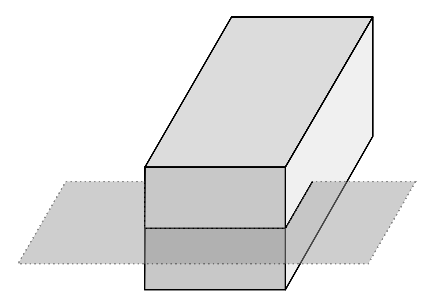
\includegraphics[width=0.7\linewidth]{Figures/Peridigm/Discretization_BondFilters_RectangularPlane}};
% Figure scope
  \begin{scope}[
    x={(image.south east)},
    y={(image.north west)},
  ]
    % Coordinates
    \coordinate (p1)  at (0.005,0.100);
    \coordinate (p2)  at (0.878,0.100);
    \coordinate (p3)  at (0.995,0.397);
    \coordinate (p4)  at (0.125,0.397);
    \coordinate (pn)  at (0.250,0.300);
    
    \coordinate (p1v) at ($(p1)-(0.0,9ex)$);
    \coordinate (p2v) at ($(p2)-(0.0,9ex)$);
    \coordinate (p2s) at ($(p2)+(1em,0.0)$);
    \coordinate (p3s) at ($(p3)+(1em,0.0)$);
    % Dots
    \draw[black,fill=black] (p1) circle (2pt);
    \draw[black]            (p2) circle (2pt);
    \draw[black]            (p3) circle (2pt);
    \draw[black]            (p4) circle (2pt);
    % Nodes
    \node[anchor=east,align=center]  at (p1) {Lower\_\\Left\_\\Corner}; 
    \node[anchor=north,xshift=0.5em] at (p1) {1}; 
    \node[anchor=north]              at (p2) {2};
    \node[anchor=south]              at (p3) {3};
    \node[anchor=south]              at (p4) {4};
    % Arrows
    \draw[-latex,very thick] (p1) -- ($(p1)+(5em,0.0)$) node [below,align=center] {Bottom\_\\Unit\_\\Vector};
    \draw[-latex,very thick] (pn) -- ($(pn)+(0.0,5em)$) node [above] {Normal};
    \draw[latex-latex,very thick] (p1v) -- (p2v) node [midway, anchor=north, align=center] {Bottom\_Length};
    \draw[latex-latex,very thick] (p2s) -- (p3s) node [midway, anchor=west, align=center,xshift=0.5em] {Side\_\\Length};
    % Labels
    \node[anchor=north east]         (modellabel) at (0.4,0.90) {Model};
    \node[anchor=north,align=center] (planelabel) at (0.8,0.03) {Rectangular\\Plane};
    \draw (modellabel) -- (0.55,0.8);
    \draw (planelabel) -- (0.82,0.2);
    % Help grid and labels
    %\pic{myimagegrid};
  \end{scope}
\end{tikzpicture}
